
\section{Prototype Implementation}

Abstract implementation overview of user and chatbot discussion.

\begin{figure}[H]
    \centering
    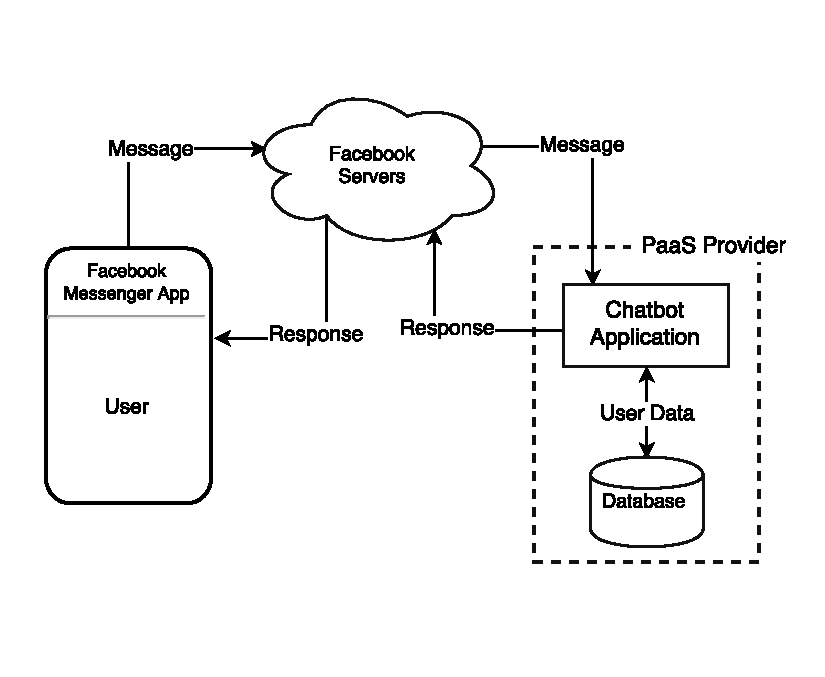
\includegraphics[width=5.1in]{../resources/diagrams/chatbot-component-overview.pdf}
    \caption{Prototype Component Overview}
    \label{fig:prototype_component_overview}
\end{figure}

\subsection{Platform}

Language consideration, nodejs, java, other types, talk about heroku, hosting provider. Hosting provider.
Database provider discussion, integration, airtable,

\subsection{Detailed Overview}

\begin{figure}[H]
    \centering
    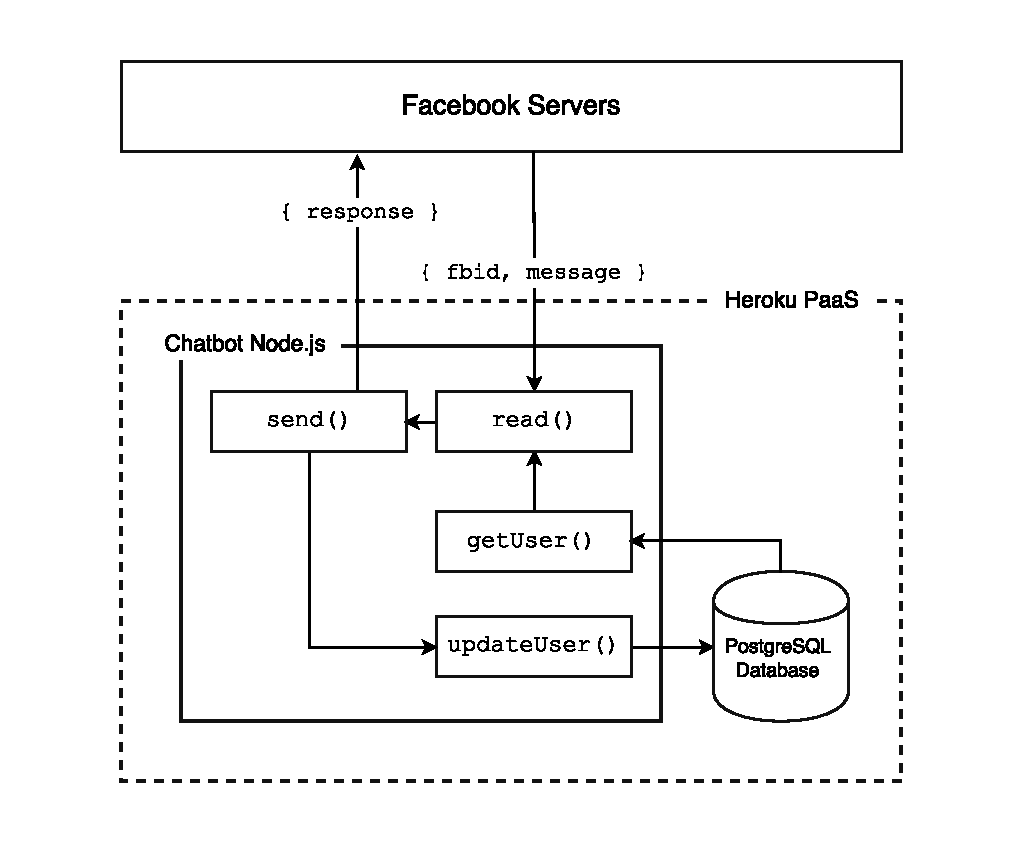
\includegraphics[width=6in]{../resources/diagrams/chatbot-detailed-overview.pdf}
    \caption{Detailed Overview}
    \label{fig:prototype_detailed_overview}
\end{figure}

Scalable architecture because heroku\newline

Implementaiton limitations about timezone with the scheduler\newline
Scheduler\newline
Free text input issues\newline

\subsection{Implementation Issues}
(Go through all meetings and list implementation issues here.)

Throughout the implementation process different techniques were explored to implement the design.
Some of the research areas were not used in the final prototype due to technical issues and limitations with the approach.\newline
\newline
Using vibration as a modality would've been a great additional modality to use.
Unfortunately the chatbot sandbox meant that the vibration ability in the phone could not be used, so another device would be used in combination with the bot.
Smart watches and fitness trackers were researched to test if they could programatically vibrate, with the pattern of vibration matching the frequency of the audio.
However, the majority of these devices did not have an API that exposed the vibration element. The best method was found to programatically set an alarm 1-minute into the future using a Fitbit fitness tracker.
This would trigger the vibration when the alarm sounded.
Although this would mean a 1-minute delay after completing a habit, a good user flow could've reduced the wait time with some additional dialogue.
But, this approach relied on the fitness tracker to sync with the phone after the alarm was programatically set. Unfortunately forcing the tracker to sync wasn't available, so this modality was abandoned.\newline
\newline
Another issue occured with stopping the audio after it had been played during a reward. If a user closed the reward box, there was no way to stop the audio, unless a user waited until it had finished. This limitation was very minor, but also showed how difficult it is to seemly connect a webview and a bot.


\subsection{Testing the chatbot}

Test harness, tested the full functionality programatically. Hooking into Travis CI and other continuous integration services.
A pilot trial tested the basic chatbot functionality. Preparing for the full evaluation trails.

\newpage